\chapter{Statistics}

%My hypothesis before start

\section{Statistics theory}


\subsection{Normal testing}\label{subsec:normaltesting}
All parametric statistics assumes normally distributed, independent observations. Parametric tests are preffered in statistics because it got more statistical power than nonparametric tests \citep{Frost2015}. The power of a test is the probability of correctly rejecting a false null hypothesis, which in this case is the ability to detect if the sample comes from a non-normal distribution. To determine if a sample is normally distrubuted there exists both visual methods and normality tests to assess the samples normality. A visual inspection of the sample's distribution is usually unreliable and does not guarantee that the distribution is normal \citep{Pearson2006}. Presenting the data visually gives the reader an opportunity to judge the distribution themselves. In this thesis histograms are used to visualize the data. 

Normality tests compare the scores in the sample to a normally distributed set of scores with the same mean and standard deviation \citep{Ghasemi2012}. There are multiple normality tests, and deciding which test to use is not easy. This study needs a test that doesn't require every value to be unique. The survey used to collect the samples in this study do not guarantee unique values. 

The D'Agostino-Pearson omnibus test stand out as the best choice. This test first computes the skewness, see figure \ref{fig:skew}, and kurtois, see figure \ref{fig:kurtois}, to quantify how far from the normal distribution the sample is from the terms of assymetry and shape. Then it calculates how far each of these values differs from the value expected with a normal distribution \citep{Pearson2006}. It works well even if all values are not unique \citep{Motulsky2013}. The test also works well on both short- and long-tailed distributions \citep{Yap2011}. \newline  %THIS STUDY HAS?? LONG OR SHORT??

\begin{figure}[h!]
	\centering
	\includegraphics[width=0.7\linewidth]{"fig/skew"}
	\caption{Skew \citep{MedCalcSoftwarebvba2017}}
	\label{fig:skew}
\end{figure}

\begin{figure}[h!]
	\centering
	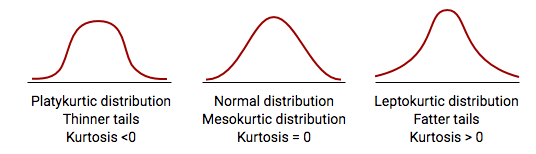
\includegraphics[width=0.7\linewidth]{fig/kurtois}
	\caption{Kurtois \citep{MedCalcSoftwarebvba2017}}
	\label{fig:kurtois}
\end{figure}


The D'Agostino-Pearson test uses the following hypothesis:\newline

\centerline{$H_{0}$: The data follows the normal distribution} 
\centerline{$H_{A}$: The data do not follow the normal distribution}

For small sample sizes, normality tests have little power to reject the null hypothesis, therefore small sample sizes most often pass normality tests. For large sample sizes, significant results would be derived even in the case of a small deviation from normality \citep{Pearson2006}. When the null hypothesis cannot be rejected, then there are two possible cases. First case is to accept the null hypothesis or the second case is that the sample size is not large enough to either accept or reject the null hypothesis \citep{ThePennsylvaniaStateUniversity2017}. An acceptance of the null hypothesis implies that the evidence was insufficient, the result does not necessary accept $H_{0}$, but fails to reject $H_{0}$ \citep{Walpole2012}.  


%A \textit{goodness-of-fit} test is used to determine whether a sample of \textit{n} observations can be considered as a sample from a given specified distribution \citep{Walpole2012}. The Anderson-Darling and the Kolmogorov-Smirow tests stand out as \textit{goodness-of-fit} procedures specialized for small samples \citep{Romeu2003}. The Anderson-Darling test will be used in this study to test if the observations gathered in this study is normally distributed.  %The Kolmogorov-Smirow test is a nonparametric test. The hypothesis for the Anderson-Darling test is: \newline

%\centerline{$H_{0}$: The data follows the normal distribution} 
%\centerline{$H_{A}$: The data do not follow the normal distribution}

%The computations in the Anderson-Darling test differs based on what is known about the observations. In this study both the expected mean and variance is unknown. In all the Anderson-Darling tests in this study a significance level of $0.05$ is used, which gives a confidence interval of $95$ \% . If the calculated \textit{p-value} is less than the significance level ($0.05$), the null hypothesis is rejected. The larger the \textit{p-value} the closer match is the data to the normal distribution. The Anderson-Darling statistics is used to calculate the \textit{p+value} for the \textit{goodness-of-fit} test. 

\subsection{Hypothesis testing}\label{sec:hypothesistesting}
The null- and alternative hypothesis are statements regarding a difference or an effect that occur in the population of the study. The alternative hypothesis (Ha) usually represents the question to be answered or the theory to be tested, while the null hypothesis ($H_{0}$) nullifies or opposes Ha \citep{Walpole2012}. The sample collected in the study is used to test which statement is most likely (technically it's testing the evidence against the null hypothesis).  When the hypothesis is identified, both null and alternative, the next step is to find evidence and develop a strategy for or against the null hypothesis \citep{LundResearchLtd2013}.

The firsy step, after identifying the hypothesis, is to determine the level of statistical significance, often expressed as the \textit{p-value}. A statistical test will result in the probability (\textit{the p-value}) of observing your sample results given that the null hypothesis is true. A significance level widely used in academic research is 0.05 or 0.01 \citep{Walpole2012}. 

%Compare the mean time in experienced and not experienced
%H0: No time difference, Ha: Experienced use less time

\subsubsection{Two sample t-test}\label{sec:t-test}
When estimating the difference between two means a two-sample t-test is used \citep{Walpole2012}. A two sampled test assumes two independent, random samples from distributions with means [$\mu_{1}$ , $\mu_{2}$] and variances [$\sigma_{1}^{2}$, $\sigma_{2}^{2}$]. %*HOW TO DETERMINE IF THEY ARE INDEPENDENT? 
The hypothesis on two means can be written as:\newline

\centerline{$H_{0}$: $\mu_{1}$ - $\mu_{2}$ = 0 or $\mu_{1}$ = $\mu_{2}$} 
\centerline{$H_{A}$: $\mu_{1}$ - $\mu_{2}$ > 0 or $\mu_{1}$ > $\mu_{1}$}
 
Then the hypothesis refer to a one-tailed two sampled t-test. Before doing tests on the two means, the Levene's Test is used to test if the samples are from populations with equal variances. It tests the hypothesis:\newline %https://docs.scipy.org/doc/scipy-0.14.0/reference/generated/scipy.stats.levene.html

\centerline{$H_{0}$: Input samples are from populations with equal variances} 
\centerline{$H_{A}$: Input samples are from populations that do not have equal variances}

If we can assume equal variances in the two samples a two-sampled t-test may be used. 
%There are also formula for Unknown but unequal variances, page 345 in statistics book

Because the one-sided tests can be backed out from the two-sided tests. (With symmetric distributions one-sided p-value is just half of the two-sided pvalue). It goes on to say that scipy always gives the test statistic as signed. This means that given p and t values from a two-tailed test, you would reject the null hypothesis of a greater-than test when p/2 < alpha and t > 0, and of a less-than test when p/2 < alpha and t < 0. %http://stackoverflow.com/questions/15984221/how-to-perform-two-sample-one-tailed-t-test-with-numpy-scipy
%https://docs.scipy.org/doc/scipy-0.18.1/reference/generated/scipy.stats.ttest_ind.html

An example of a relevant hypothesis test neccessary in this study is:\newline
\centerline{$H_{0}$:  $\mu_{E} =  \mu_{N} $} 
\centerline{$H_{A}$: $\mu_{E} > \mu_{N}$}

Where $\mu_{E}$ is the mean task time for experienced participants and $\mu_{N}$ is the mean task time for non-experienced participant's. More on this later. %*WHICH SECTION?

\subsubsection[ANOVA]{Analysis-of-Variance}\label{sec:anova}
Analysis-of-Variance (\textit{ANOVA}) is according to \cite{Walpole2012} a very common procedure used for testing population means. A part of the goal of \textit{ANOVA} is to determine if the differences among the sample means are what we would expect due to random variation alone, or due to variation beyond merely random effects. \textit{ANOVA} assumes normally distributed samples with equal variance. 

One-way \textit{ANOVA} is used to determine if three or more independent groups have any significant differences between their means.  It tests the hypothesis:\newline

\centerline{$H_{0}$:  $\mu_{1} =  \mu_{2} = ... = \mu_{k} $} 
\centerline{$H_{A}$:  At least two of the means are different}

$\mu$ equals the group mean and $k$ represents the number of groups. The weakness of one-way \textit{ANOVA} is that it cannot tell which specific groups were significally different from each other if $H_{0}$ is rejected. To be able to determine which group a \textit{post hoc test} is used. 

In this test there should be one variable and minimum three groups, which is an relevant approach considering the data produced from the survey. The test can determine if the mean time (the variable) is significally different between the three tasks (the groups) given in the survey. It can also be used to determine if there are any significant different in mean time given the six different orders the task could serve in. A third test is to have number of correct elements as the variable and the three tasks as groups. More on this later. %*WHIch section?






